\documentclass[10pt,pdf,hyperref={unicode}]{beamer}
\usetheme{Berlin}
\usepackage{graphicx}

\usepackage[utf8]{inputenc}
\usepackage[T1,T2A]{fontenc}
\usepackage{microtype}
\beamertemplatenavigationsymbolsempty

\usepackage[russian, english]{babel}
%----TITLE INFO BEGIN-----
\title[Исследование сечений тессеракта трехмерной гиперплоскостью с использованием методов компьютерного моделирования] % ( long titles)
{ \bfseries Исследование сечений тессеракта гиперплоскостью}
\subtitle{используя методы компьютерного моделирования.}

\author[Максимов Г., Нугманов А., Мустафин И.]
{ \bfseries Максимов Григорий, Нугманов Артур, Мустафин Ильгиз}

\institute[ТТЛ №2] % (optional)
{
  { \normalsize Татаро - Турецкий Лицей №2} \\
  Московского района города Казани
}

\date[2015-03-26] % (optional)
{Конференция имени Лобачевского 2015}
\subject{Математика}
%-----TITLE INFO END-----

\begin{document}
\frame{\titlepage}

\begin{frame}
\frametitle{Тессеракт. Общее определение}

\begin{columns}
	\column{0.5\textwidth}
		\framebox{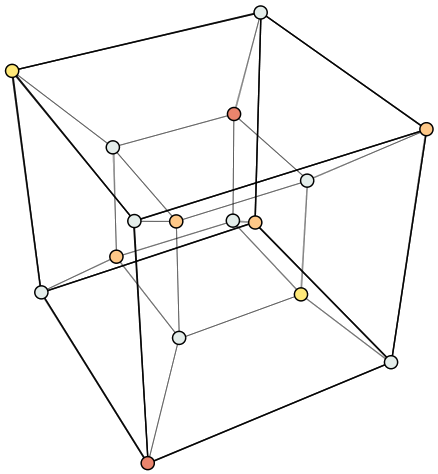
\includegraphics[scale=0.3]{./tesseract_fig1.png}}
	\column{0.5\textwidth}
	{\small
	\begin{itemize}
		\item Рассматриваемая нами модель имеет координаты $(x_1,x_2,x_3,x_4) \in R^4$, такие, что $x_1 \in [ -1,1 ]$. 
		\item Ограгичивается 8 гиперплоскостями	
		\item Имеет 8 трехмерных граней, 24 двумерных, 32 ребра и 16 вершин.
	\end{itemize}
}
	\clearpage
\end{columns}

%\begin{columns}
%		\column{0.5\textwidth}
% 			Содержимое левого столбца
% 		\column{0.5\textwidth}
% 			Содержимое правого столбца
%\end{columns}
\end{frame}
\begin{frame}
\frametitle{Наглядный процесс формирования отображения тессеракта на трехмерную плоскость}
\begin{center}
\framebox{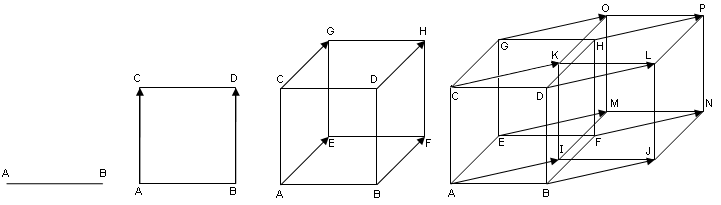
\includegraphics[scale=0.4]{./make_tess.png}}
\end{center}
\\

Наглядный процесс, как точка $A$ переходит постепенно в гиперкуб, приобретая новые размерности
\end{frame}
\begin{frame}
	%THESIS
	Раскрытие тезиса здесь.
\end{frame}
\begin{frame}
	\frametitle{Лемма о размерности сечений}
{\small
	\begin{block}{Утверждение}
		Сечение любого $4$-мерного геометрического объекта $3$ мерной гиперплоскостью есть геометрическое тело, имеющее размерность не более $3$. 
	\end{block}
}
	\begin{columns}
		\column{0.5\textwidth}
			\framebox{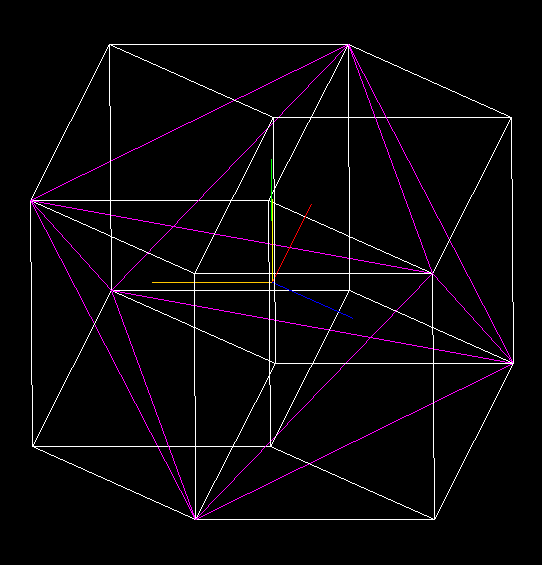
\includegraphics[scale=0.25]{./a3.png}}
		\column{0.5\textwidth}
			\framebox{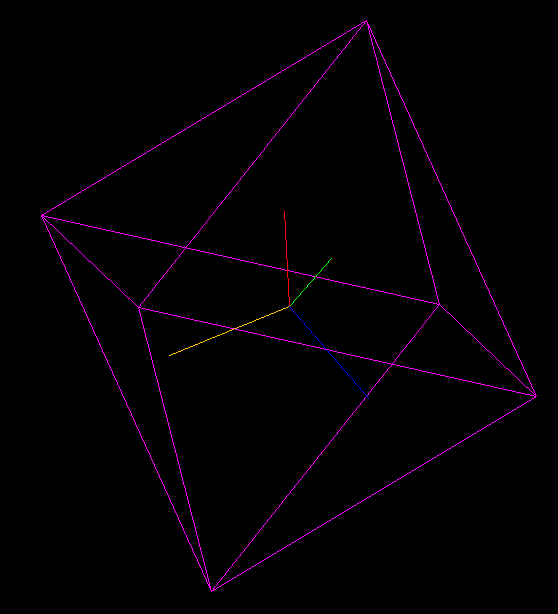
\includegraphics[scale=0.2]{./a4.png}}
	\end{columns}
\end{frame}
\begin{frame}
	\frametitle{Метод построения сечений тессеракта гиперплоскостью}
	\begin{itemize}
		\item Задать гиперплоскость сечения
		\item Найти точки пересечения гиперплоскости и тессеракта
		\item Повернуть получившееся сечения до вложимости его в трехмерное пространство
		\item Вывод полученного сечения, анализ результатов
	\end{itemize}
	\framebox{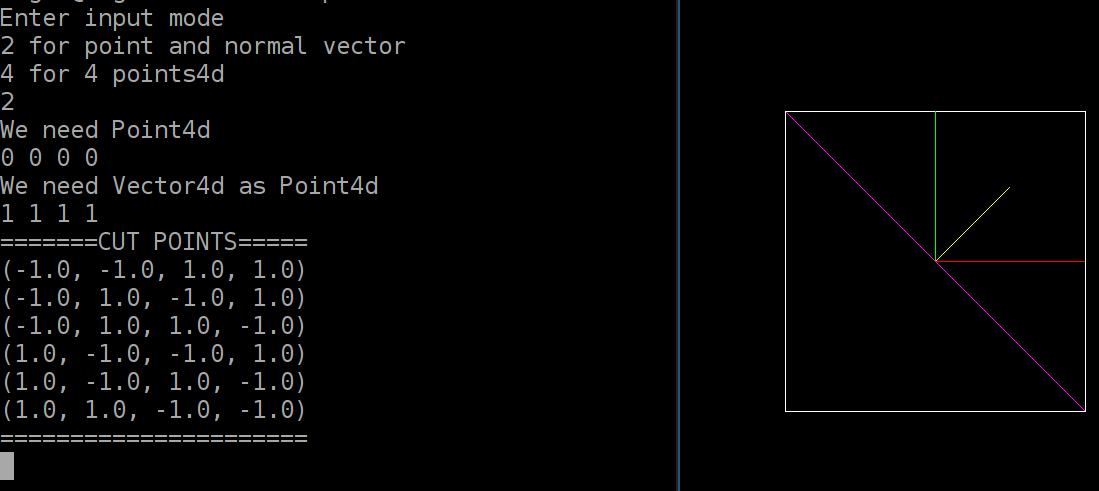
\includegraphics[scale=0.26]{./a1.png}}
\end{frame}
\begin{frame}
	\frametitle{Задание гиперплоскости сечения}
	\begin{block}{Гиперплоскость сечения. Уравнение.}
		{\bfseries $ax+by+cz+dw+e=0$} \\ $(a,b,c,d,e)$ - коэффициенты\\  $(x,y,z,w)$ - координаты точек.
	\end{block}
	Задается по четырем точкам с помощью матрицы: \\

	\begin{flushleft}
	$$ \left|
	\begin{array}{cccc}
		x-x_1 & y-y_1 & z-z_1 & w-w_1     \\
		x_2-x_1 & y_2-y_1 & z_2-z_1 & w_2-w_1    \\
		x_3-x_1 & y_3-y_1 & z_3-z_1 & w_3-w_1      \\
		x_4-x_1 & y_4-y_1 & z_4-z_1 & w_4-w_1 
	\end{array}
	\right|=0
	$$
\end{flushleft}
						
 Таким образом, мы объявили гиперплоскость сечения.

\end{frame}
\begin{frame}
	\frametitle{Задание гиперплоскости с помощью точки и вектора}
	\begin{block}
		$$
		A(x_1,y_1,z_1,w_1) \mbox{ - произвольная точка} \\
		\overrightarrow N (x_2,y_2,z_2,w_2) \mbox{ - нормаль к искомой гиперплоскости} \\
		P(ax+by+cz+dw+e=0) \\
		e=-(x_2x_1+y_2y_1+z_2z_1+w_2w_1)
		$$
\end{block}
Таким образом, мы задали гиперплоскость, используя точку и вектор.
\end{frame}
\begin{frame}
	\frametitle{Нахождение точки пересечения гиперплоскости и тессеракта}
	Пусть $A$ - вершина гиперкуба, $P$ - наша гиперплоскость. \\
	Произведем проверку взаимного расположения вершины тессеракта и гиперплоскости.\\
	\begin{block}{}
	$
		A:=(x_1,y_1,z_1,w_1) \\
		P:=(ax + by + cz + dw + e = 0) \\
		\left[
		\begin{array}{cc}
			ax_1 + by_1 + cz_1 + dw_1 + e = 0 & \mbox{Вершина принадлежит сечению} 
			\\
			ax_1 + by_1 + cz_1 + dw_1 + e > 0 & \mbox{Вершина "выше" плоскости сечения}
			\\
			ax_1 + by_1 + cz_1 + dw_1 + e < 0 & \mbox{Вершина "ниже" плоскости сечения} 
		\end{array}
	$
\end{block}
\\

Далее при помощи параметрического уравнения находим точку пересечения. Надо дописать.
\end{frame}
\begin{frame}
	\frametitle{Поворот сечения}
	\\

	\begin{columns}
		\column{0.5\textwidth}
	\begin{block}{Матрицы поворота в четырехмерном пространстве.}
		{\footnotesize
			$$
			M_{xy}(\alpha)=
			\left(
			\begin{array}{cccc}
				\cos \alpha & -\sin \alpha & 0 & 0 \\
				\sin \alpha & \cos \alpha & 0 & 0 \\
				0 & 0 & 1 & 0 \\
				0 & 0 & 0 & 1
			\end{array}\right)
			$$
			\\
			
			\newline
			$$
			M_{yz}(\alpha)=
			\left(
			\begin{array}{cccc}
				1 & 0 & 0 & 0 \\
				0 & \cos \alpha & -\sin \alpha & 0 \\
				0 & \sin \alpha & \cos \alpha & 0 \\
				0 & 0 & 0 & 1
			\end{array}\right)
			$$	
			\\ 

			$$
			M_{zw}(\alpha)=
			\left(
			\begin{array}{cccc}
				1 & 0 & 0 & 0 \\
				0 & 1 & 0 & 0 \\
				0 & 0 & \cos \alpha & -\sin \alpha \\
				0 & 0 & \sin \alpha & \cos \alpha
			\end{array}\right)
			$$
		}

\end{block}
\column{0.5\textwidth}
PIC HERE
\end{columns}
\end{frame}
\begin{frame}
	\frametitle{Лемма о выпуклости}
	\begin{block}{Лемма 1}
		Сечением выпуклого тессеракта гиперплоскостью является выпуклое геометрическое тело.
	\end{block}
\end{frame}
\end{document}
